\documentclass[a4paper]{article}
\usepackage[warn]{mathtext}
\usepackage[utf8]{inputenc}
\usepackage[T2A]{fontenc}

\usepackage[english,russian]{babel}
\usepackage{multicol}
\usepackage{fancyhdr}
\usepackage{graphicx}
\usepackage{microtype}
\usepackage{wrapfig}
\usepackage{amsmath}
\usepackage{floatflt}
\usepackage{geometry} \geometry{verbose,a4paper,tmargin=2cm,bmargin=2cm,lmargin=1.5cm,rmargin=1.5cm}
\usepackage{float}
\usepackage{amssymb}
\usepackage{caption}
\usepackage{epsfig}
\usepackage{newunicodechar}

\begin{document}

\graphicspath{ {pictures/} }

\begin{titlepage}
	\centering
	\vspace{5cm}
    {\scshape\LARGE Московский физико-технический институт\par}
	\vspace{5cm}
	{\scshape\Large Лабораторная работа по общей физике \par}
	\vspace{1cm}
    {\huge\bfseries  №11.5 Туннелирование в полупроводниках  \par}
	\vspace{1cm}
	\vfill
    \begin{flushright}
        {\large выполнил студент Б04-852 группы ФЭФМ}\par
        \vspace{0.3cm}
        {\LARGE Яромир Водзяновский}
    \end{flushright}
	\vfill
Долгопрудный, 2021
% Bottom of the page
\end{titlepage}

\pagestyle{fancy} 
\fancyhead[L]{Туннелирование   $\sim  \hat(\, ^{\circ}  \omega  ^{\circ} \, \hat) \sim$}
% \fancyhead[L]{Закон Кюри-Вейса    $( *{^\circ}< >^{\circ}*)$}
\fancyhead[R]{Современная физика}
\fancyfoot[C]{ \noindent\rule{\textwidth}{0.4pt} \thepage }

\tableofcontents

\newpage



\section{Цель работы}

Исследовать принцип действия туннельного диода, измерить его ВАХ и основные параметры.


\section{Теория}

Туннелирование в полупроводниках обусловлено тем, что магнитные и электрические св-ва полупровдников можно менять в широких пределах, добавляя примеси. 
Эффективные массы электронов в полупроводниках меньше массы свободного электрона и туннелирвоание идет на более дальние расстояния.  \par 

Электроны в кристаллах движутся в периодической решетке ионов и свободное движение жлектрона не означает <<свободу>> электрона. Заряд при движении остается преждним, а
соотношение между импульсом и кинетической энергией меняется.  \par 

Введение в полупрводник примесей приводит к появленб разрешенных уровней в запрещенной зоне, между которыми происходит обмен электронами. 
Примеси, дающие уровни вблизи нижнего края зоны проводимости, называются донорными. Для кремния или германия донорными являются элементы 5-й группы: P, As, Sb.
При щамещении одного из атомов Si, As только 4 из 5 электронов оказываются в решетке, 5-й остается <<лишним>>. Уровень этого электрона находится вблизи дна зорны проводимости $\sim -0.01\; эВ$. 
Мы получили пролупровдник n-типа. \par 

Если в кремний ввести элементы 3-й группы: B, Al, Ga, In, то часть электронов с валентной зоны перейдет на близь лежащие уровни в запрещенной зоне. Теперь у нас будет недостаток одного электрона, что и создаст дополнительные уровни. 
Расстояние локальных уровней от начала зщапрещенной зоны составляет $0.01\;  эВ$, и возможны переходы при комнатнгой температуре $0.025\; эв$. Мы получили полупровдник p-типа. \par 

Сильно легированный проводник n-типа появляется целая полоса электронов на дне зоны проводимости, а у p-полупроводника образовалась полоса свободных состояний у потолка валентной зоны, таким образом, 
в сильно легированных полупроводниках в области узкого p-n перехода становятся вощможны туннельные переходы электронов, поэтому диод так называется. \par 

В вырожденном полупровднике уровень Ферми для n-типа лежит в зоне провдимости, а для p-типа в валентной зоне. Расстояние от Ферми до краев зон: 
$$\xi = \mu_n - E_c \;\;\;\;\;\; \eta = \mu_p - E_v$$

В отсутвии внешнего поля (рис. \ref{cheme}а) нет тока в диоде, тк уровни $\mu_p$ и $\mu_n$ лежат в одной горизонтали и нет перекрытия своодных занятых состояний. \par 

Если приложить поле (рис. \ref{cheme}б), те плюс к p-области, то в этом случае внешнее поле будет противополжно внутреннему в переходе. Если увеличивать внешнее поле, то смещение зон уменьшится, и часть областей перекроется и будет ток, электроны туннелируют налево. \par 

При дальнейшем увеличении внешнего поля ток достигнет максимума (точка б на ВАХ) и начнет спадать (точка в на ВАХ), тк зона провдимости поднимается. В дальнейшем вообще пропадет ток (точка г на ВАХ), тк не будет пересечения дна зоны проводимости с валентной зоной. При напряжении 
$U = (\xi + \eta)/e$ ток полностью прекращается (рис. \ref{cheme}г). При дальнейшем увеличении напряжения занятые уровни n-области начинают совпадать с незанятыми уровнями в зоне проводимости, аналогично и свободные уровни p-области сопадают с занятыми уровнями в ванетной зоне (рис. \ref{cheme}д). 
Это называется \textbf{диффузионный ток}, уже нет туннелирования, ток резко возрастает. \par 

При обратном напряжении (рис. \ref{cheme}е) уровень Ферми $\mu_p$ смещается вверх относительно $\mu_n$ и при этом против заселенных состояний в p-области появляются свободные уровни в n-области. Электроны p-полупроводника туннелируют в n-полупроводник, течет ток, обусловленный 
неосновными носителями и ток будет в обратном направлении.  \par 

Реальная ВАХ отличается от изораженной на (рис. \ref{cheme}ж) и выглядит следующим образом (рис. \ref{p2}). Она зарактеричзуется основными параметрами:

\begin{enumerate}
    \item $U_p$ соответсвует максимуму тока $I_p$.
    \item $U_v$ соответсвует минимальному току $I_v$.
    \item $U_f$ $(|U_f > U_v|)$, при которой ток равен $I_p$.
\end{enumerate}



\begin{figure}[h]
    \begin{center}
        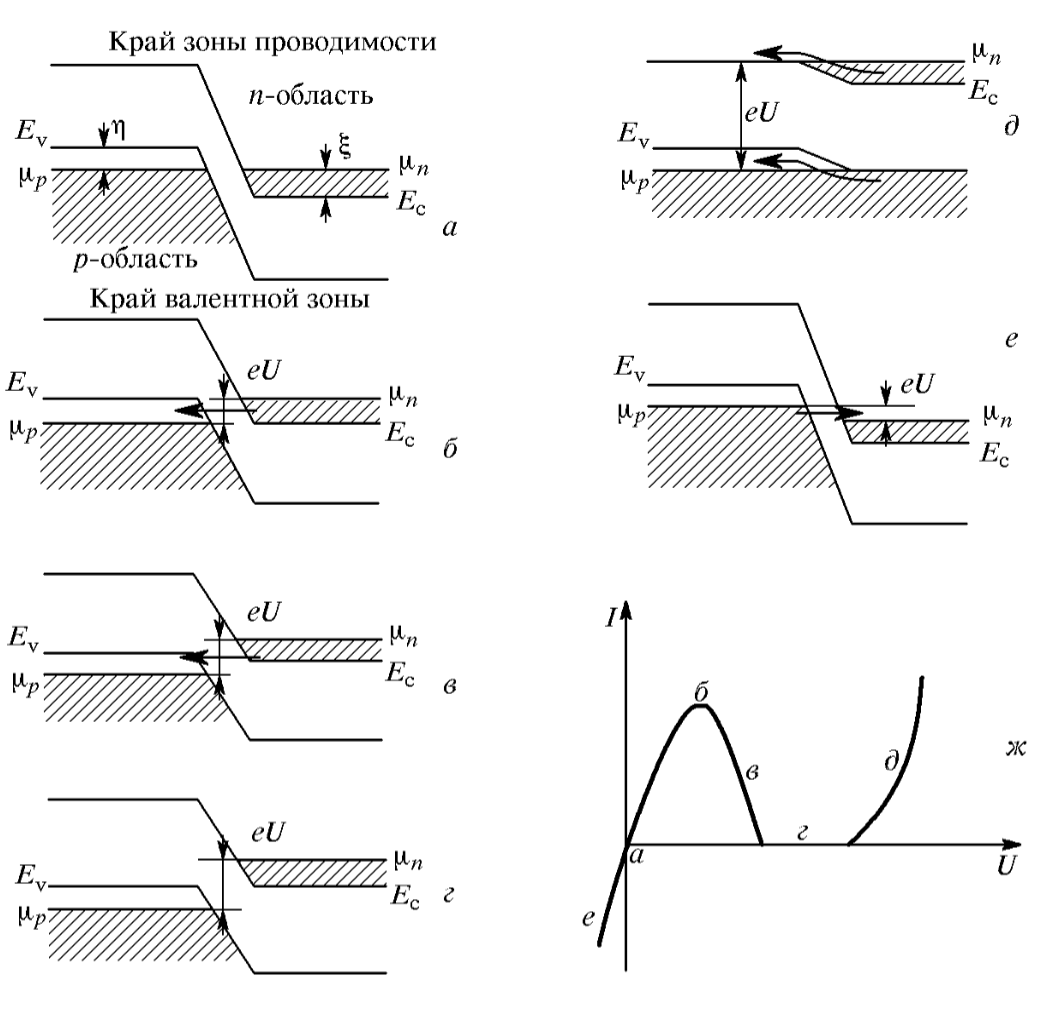
\includegraphics[scale = 0.8]{cheme.png}
        \caption{Схема энергетических уровней и ВАХ идеального туннельного диода}
        \label{cheme}
    \end{center}
\end{figure}

\begin{figure}[h]
    \begin{center}
        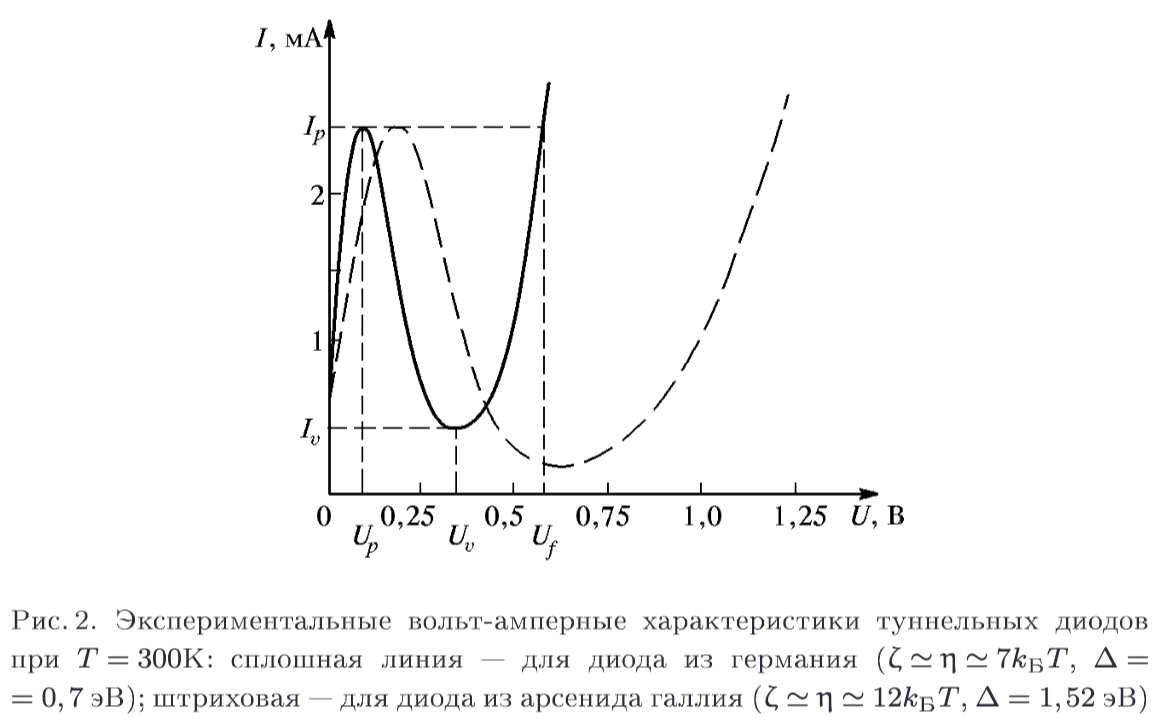
\includegraphics[scale = 0.6]{p2.png}
        \caption{}
        \label{p2}
    \end{center}
\end{figure}

Наличие тока на участке между туннельной и диффузионной ветвями обуславливается: 
\begin{itemize}
    \item Образованием примесных зон из-за большой концентрации донорных центров в 
    n-полупроводнике и акцепторных центров в p-полупровднике. Мелкие примесные уровни могут сливаться с основными зонами. 
    В результате переходов из примесных зон возрастает ток $I_v$, а $U_v$ увеличивается до значения $U = (\xi + \eta + E_d + E_a)/e$, $E_d$ и $E_a$ - ширина донорной и акцепторной зон. 
    \item Вклад в ток дает увеличенная концентрация глубоких примесей, что приводит дополнительным пикам тока на ВАХ. По положению этих пиков можно оценить энергию ионизации примесей. 
\end{itemize}

Мы полагали, что выше уровня Ферми нет электронов. При конечной температуре $T$ распределение Ферми $f(E)$ размывается на величину порядка $2k_bT$. Плотность энергетических состояний $g(E)$ неодинакова в зоне: вблизи 
границы уровни реже. Плотность заполнения уровней:

\begin{equation}
    n(E) = f(E)g(E)
\end{equation}

Уровень Ферми отстоит от краев зон на $E_F \approx \mu_n \approx \mu_n \approx k_bT$. Если подавать прямое напряжение на переход, то зоны будут смещаться. При достижении $U_v$ ток через диод минимален, что соответсвует совпадению 
границ зон проводимости $E_c$ и валентной зоны $E_v$. Отсюда оценим положение уровней Ферми:

\begin{equation}
    U_v \approxeq \frac{\xi + \eta}{e}
\end{equation}

Если оба полупроводника вырождены одинаково, то:

\begin{equation}
    U_v \approxeq \frac{2 \xi}{e} \approxeq \frac{2 \eta}{e}
\end{equation}

Напряжению $U_p$ соответсвует пик $I_p$, при котором смещение энергетических зон одинаково, точки на графиках $n(E)$ и $p(E)$ оказались на одной горизонтали. 
Так мы определим энергетический промежуток между уровнем Ферми и максимум плотности распределения электронов $n_{max}(E)$:

\begin{equation}
    U_p \approxeq \frac{\xi - E_{n \; max}}{e}
\end{equation}

Напряжение $U_f$ характеризует раствор ВАХ, определяется шириной запрещенной зоны. Напряжение $U_f$ для каждого из диодов оличается во столько раз, во сколько раз отличается ширина запрещенной зоны. 
На рис. \ref{p2} видно, что напряжения $U_f$ для каждого из диодов отличается во столько раз, во сколько отличается ширина запрещенной зоны. \par 

<<Прикол>> диода заключается в отрицательности дифференциаольного сопротивления $dU/dI$ в интервале от $U_p$ до $U_v$ и диод работает как активный элемент. Его используют как микроволновый генератор.


\section{Ход работы}

\subsection{Изучение ВАХ с помощью осциллографа}

Схема для наблюдения ВАХ на рис. \ref{osc}. На вход Y подается напряжение пропорциональное току, протекшему через диод, а на вход 
X - падение напряжения на диоде. На одну диагональ моста подается переменное напряжение отзвукового генератора через диод (исключает большые обратные токи через туннельный диод).

\begin{figure}[H]
    \begin{center}
        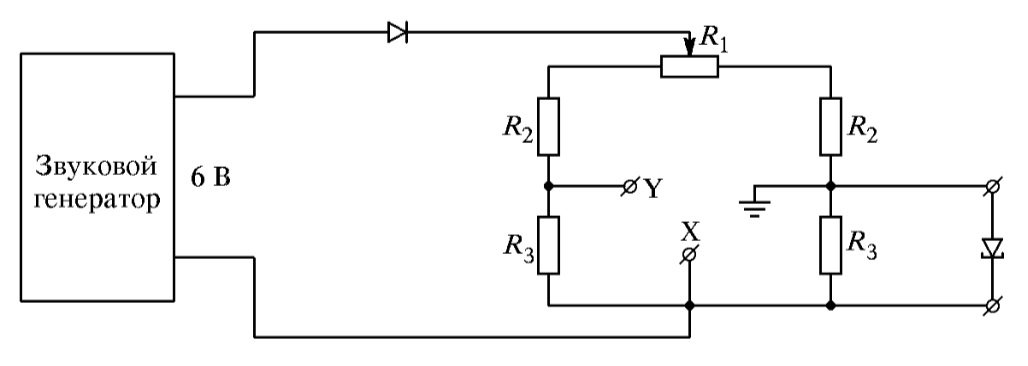
\includegraphics[scale = 0.8]{osc.png}
        \caption{Принципиальаня схема наблюдения ВАХ туннельного диода с помощью осциллографа}
        \label{osc}
    \end{center}
\end{figure}

Формула тока:

\begin{equation}
    I_д = U_Y \frac{R_1 + 2(R_2 + R_3)}{(R_1 + R_2)R_3}
    \label{cur}
\end{equation}

где $R_1 = 680 \; \Omega, \;\; R_2 = 100 \; \Omega, \;\; R_3 = 120 \; \Omega$

\begin{figure}[H]
    \begin{center}
    \begin{minipage}[h]{0.45\linewidth}
        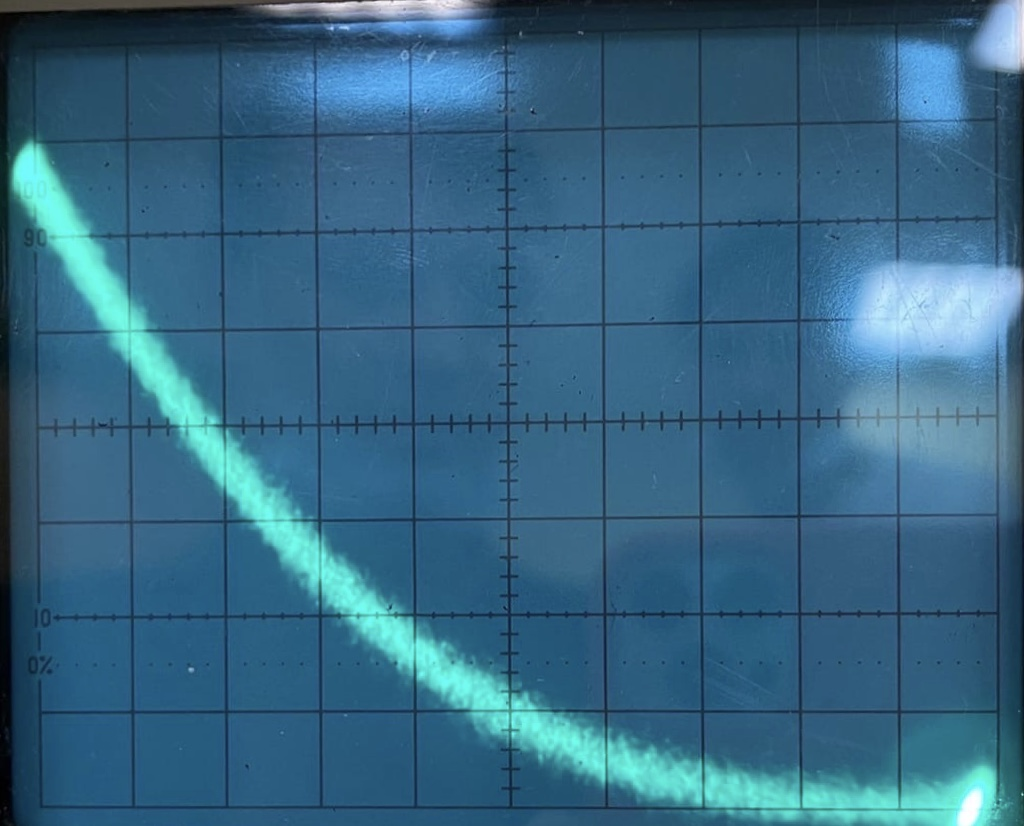
\includegraphics[width=1\linewidth]{vah1.jpg}
        \caption{ВАХ обычного полупроводникового диода. X = 0.5 В, Y = 20 мВ}
        \label{vah1}
    \end{minipage}
    \hfill 
    \begin{minipage}[h]{0.45\linewidth}
        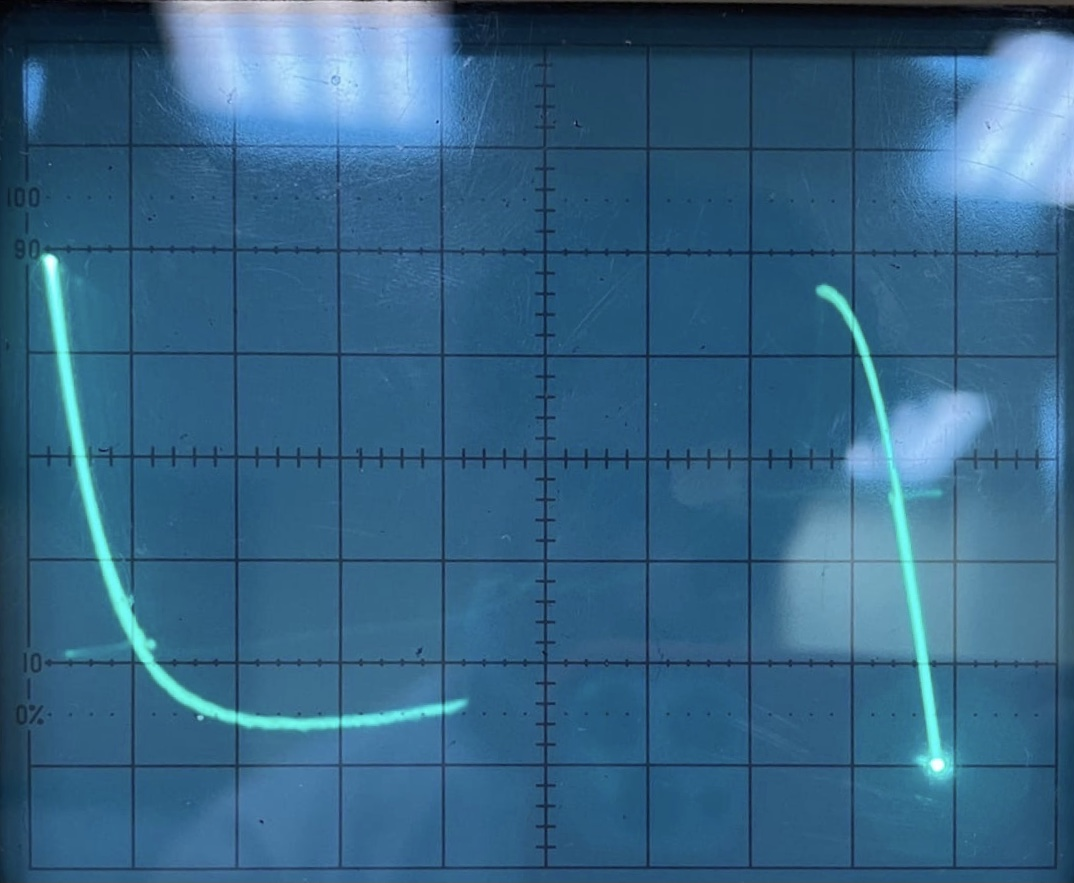
\includegraphics[width=1\linewidth]{vah2.jpg}
        \caption{ВАХ туннельного диода. X = 10 мВ, Y = 0.1 В}
        \label{vah2}
    \end{minipage}
    \end{center}
\end{figure}

\begin{itemize}
    \item По ВАХ рис. \ref{vah2} измерим характерные значения напряжений $U_p,\; U_v,\;U_f$:

    \begin{table}[H]
        \begin{center}
            \vspace{0.1cm}
            \begin{tabular}{|c|}
                \hline
                $U_p = 5\cdot 10mB = 0.05 \pm 0.01\;B$ \\ 
                $U_v = 31\cdot 10mB = 0.31 \pm 0.01\;B$ \\
                $U_f = 44 \cdot 10mB =  0.44 \pm 0.01 \;B$ \\
                \hline
            \end{tabular}
        \end{center}
    \end{table}

    \item По формуле (\ref{cur}) определим токи:
    
    \begin{table}[H]
        \begin{center}
            \vspace{0.1cm}
            \begin{tabular}{|c|}
                \hline
                $I_p = 0.53 \pm 0.11\; mA$ \\ 
                $I_v = 3.29 \pm 0.11 \; mA$ \\
                \hline
            \end{tabular}
        \end{center}
    \end{table}

\end{itemize}


\subsection{Изучение ВАХ статически}

\begin{enumerate}
    \item соберем схему на рис. \ref{stat}, туннельный диод вставим в схему последним, ручка потенциометра $R$ в минимальное положение. 
        \begin{figure}[H]
            \begin{center}
                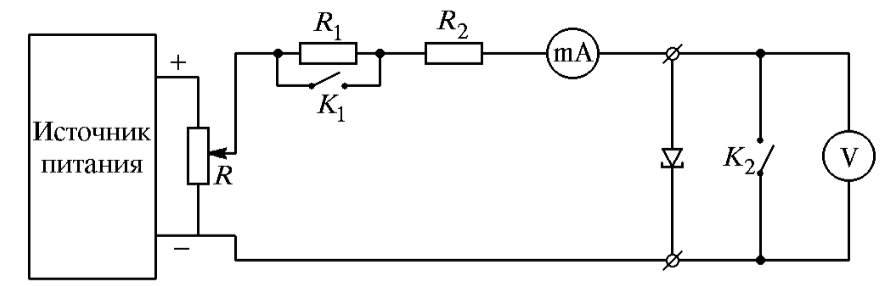
\includegraphics[scale = 0.8]{stat.png}
                \caption{Принципиальаня схема измерения параметров ВАХ туннельного диода}
                \label{stat}
            \end{center}
        \end{figure}
    \item Включим миллиамперметр и вольтметр.
    \item Плавно повышая напряжение на диоде изменением $R$ реостата ($K_1,\; K_2$ разомкнуты) снимем показания вольтметра и миллиамперметра.
    \item Занесем данные в таблицу на рис.  \ref{data}, построим ВАХ $I(U)$ на рис. \ref{gr1} 
        \begin{figure}[H]
            \begin{center}
                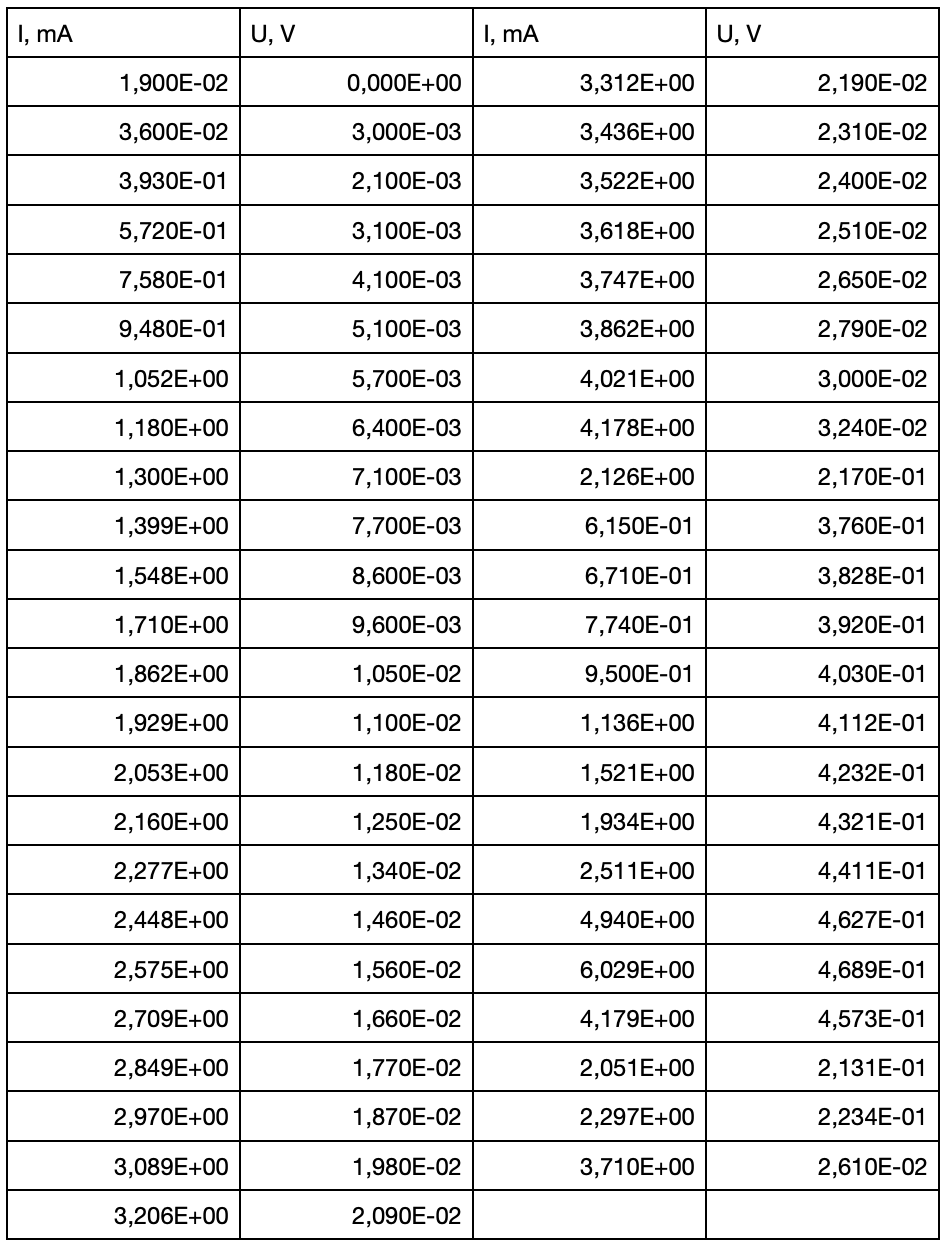
\includegraphics[scale = 0.8]{data.png}
                \caption{Данные статического эксперимента}
                \label{data}
            \end{center}
        \end{figure}
        
        \begin{figure}[H]
            \begin{center}
                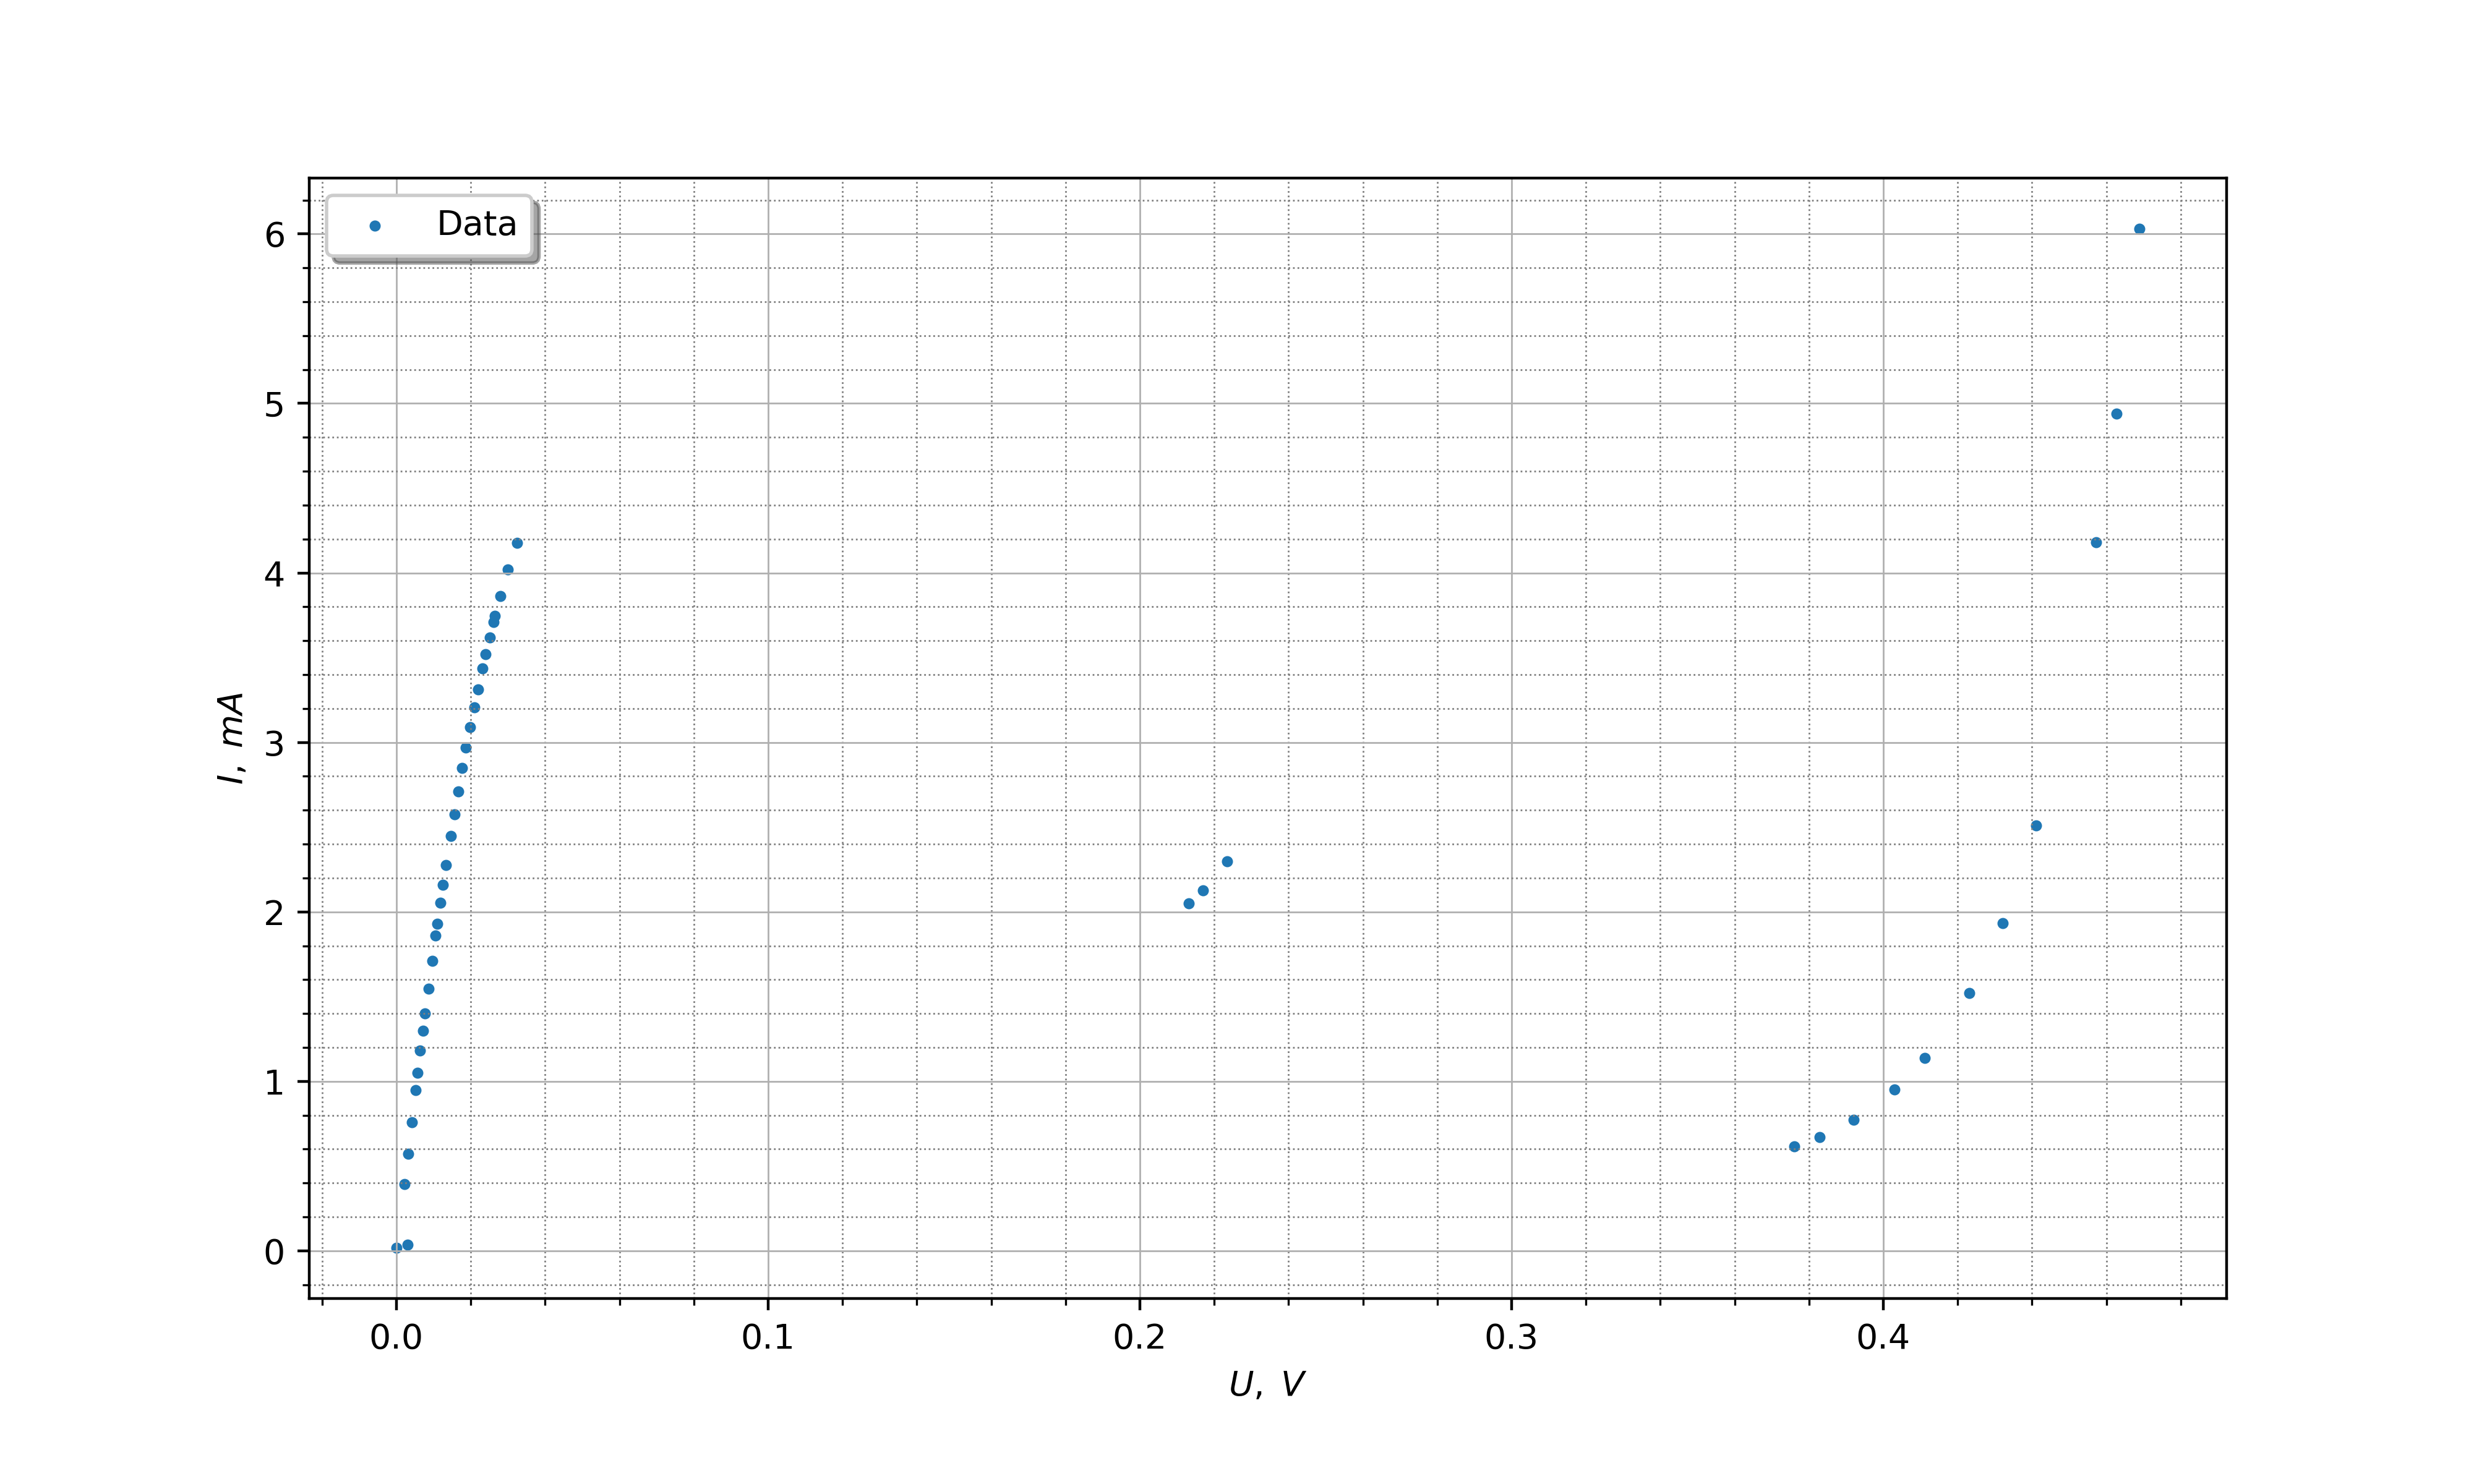
\includegraphics[scale = 0.8]{graph1.png}
                \caption{}
                \label{gr1}
            \end{center}
        \end{figure}
    \item По графику ВАХ (рис. \ref{gr1}) определим значения напряжений $U_v,\; U_p, \; U_f$ и токов $I_v, \; I_p, \; I_f$.
        \begin{table}[H]
            \begin{center}
                \vspace{0.1cm}
                \begin{tabular}{|c c|}
                    \hline
                    $U_p = 0.032 \pm 0.001\;B$ & $I_p = 4.18 \pm 0.01\; mA$ \\ 
                    $U_v = 0.376 \pm 0.001\;B$ & $I_v = 0.62 \pm 0.01\; mA$ \\
                    $U_f = 0.457 \pm 0.001\;B$ & $I_f = 4.18 \pm 0.01\; mA$ \\
                    \hline
                \end{tabular}
            \end{center}
        \end{table}

    \item Оценим положения уровня Ферми $\mu_n$ и максимума $n_{max}(E)$ расппределения электронов в зоне проводимости по формулам (3), (4) и 
    полученным значениям $U_p,\; U_v$:
    $U_v$ соответсвует минимуму тока, когда уровни $E_v=E_c$ совместились, примем тогда $E_v=0$, тогда из выражения (3):
    \begin{center}
        \fbox{$\mu_n \approx \mu_p \approx eU_v/2 \approx  0.188 \pm 0.001\; эВ$}
    \end{center}
    Из выражения (4) получим $E_{n\; max}$:
    \begin{center}
        \fbox{$E_{n\; max} = \mu_n - eU_p \approx 0.156 \pm 0.002\; эВ$}
    \end{center}
\end{enumerate}


\subsection{Генератор на основе туннельного диода}

\begin{enumerate}
    \item Соберем схему генератора (рис. \ref{gen}). Диод поключим последним в очередь.

        \begin{figure}[h]
            \begin{center}
                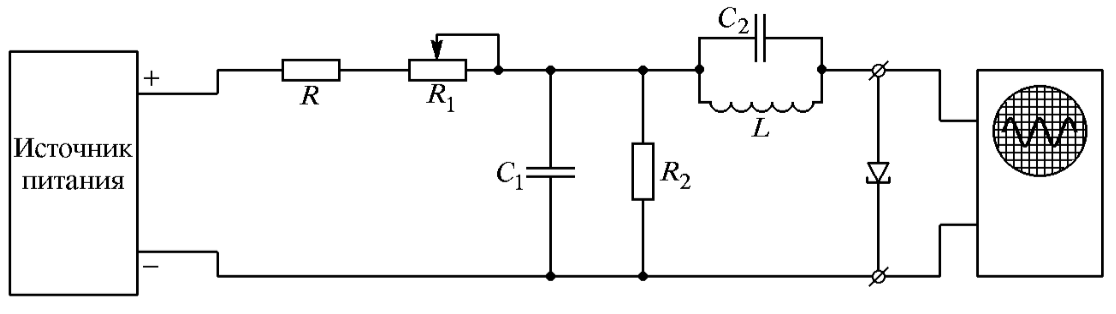
\includegraphics[scale = 0.8]{gen.png}
                \caption{Принципиальная схема генератора на туннельном диоде}
                \label{gen}
            \end{center}
        \end{figure}

    \item Включим осциллограф и источник постоянного тока в сеть.
    \item Изменяя сопростивление $R$ перемещая рабочую точку диода на спадающий участок ВАХ получим генерацию (рис. \ref{gen1})

    \begin{figure}[H]
        \begin{center}
            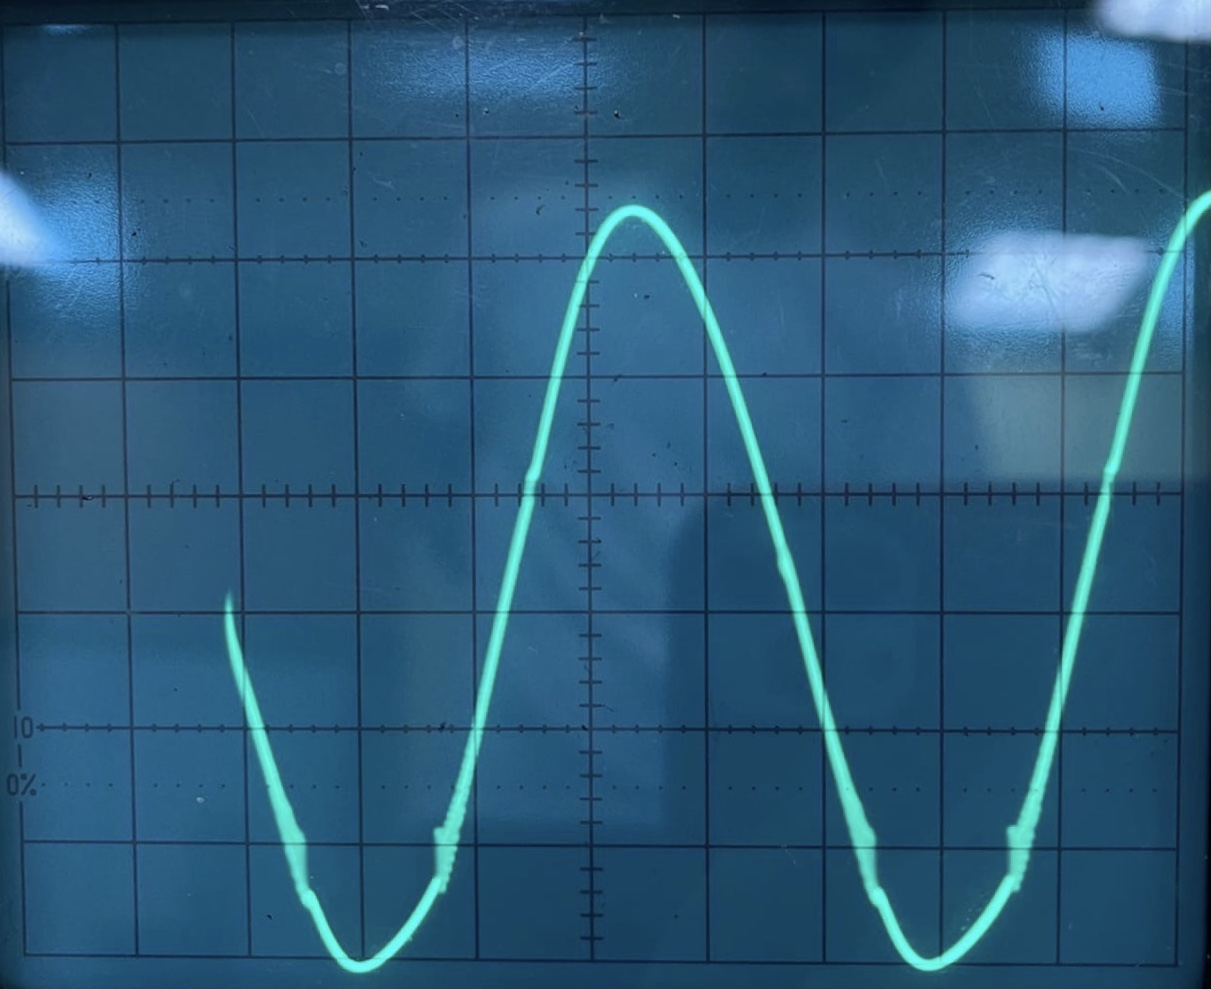
\includegraphics[scale = 0.2]{gen1.jpg}
            \caption{Генерация от гуннельного диода на осциллографе. Х = 50 мВ, Y = 0.1 В}
            \label{gen1}
        \end{center}
    \end{figure}

\end{enumerate}


\section{Вывод}
В работе исследован принцип дейтсвия туннельного диода. Наблюдали ВАХ на осциллографе, получили ее в статичеком режиме, снимая зависимость тока от напряжения. Также 
получили основные параметры и по ним рассчитали положение уровня Ферми.

\end{document}